\section{Method}
\label{sec:method}


There are different diffusion frameworks, including DDPM \cite{ho_denoising_2020} and
DDIM \cite{song_denoising_2022}, which involve a denoising network $\varepsilon_\theta$ whose
architecture is generally independent of the diffusion parameters. We will focus more on the network
architecture than on the diffusion process itself, as no contribution is made to the latter. Note that
the authors of the paper used the DDIM framework so as to be able to use a different number of denoising
iterations in training and inference, which allows for a faster sampling process at test time.

At timestep t, let $A_t$ be the action sequence and $O_t$ the observation.
% (which may contain several previous images of the scene and the end-effector pose).
The observation may contain features from several previous images of the scene, extracted by a trainable
ResNet encoder, and the end-effector pose. This observation vector is seen as a conditioning input
to guide the action sequence generation. Once the action sequence is generated, the agent executes only a
subset of it, in a receding horizon fashion.
Two architectures are proposed for the denoising network (Figure \ref{fig:diffusion_policy}).
\begin{figure*}
    \centering
    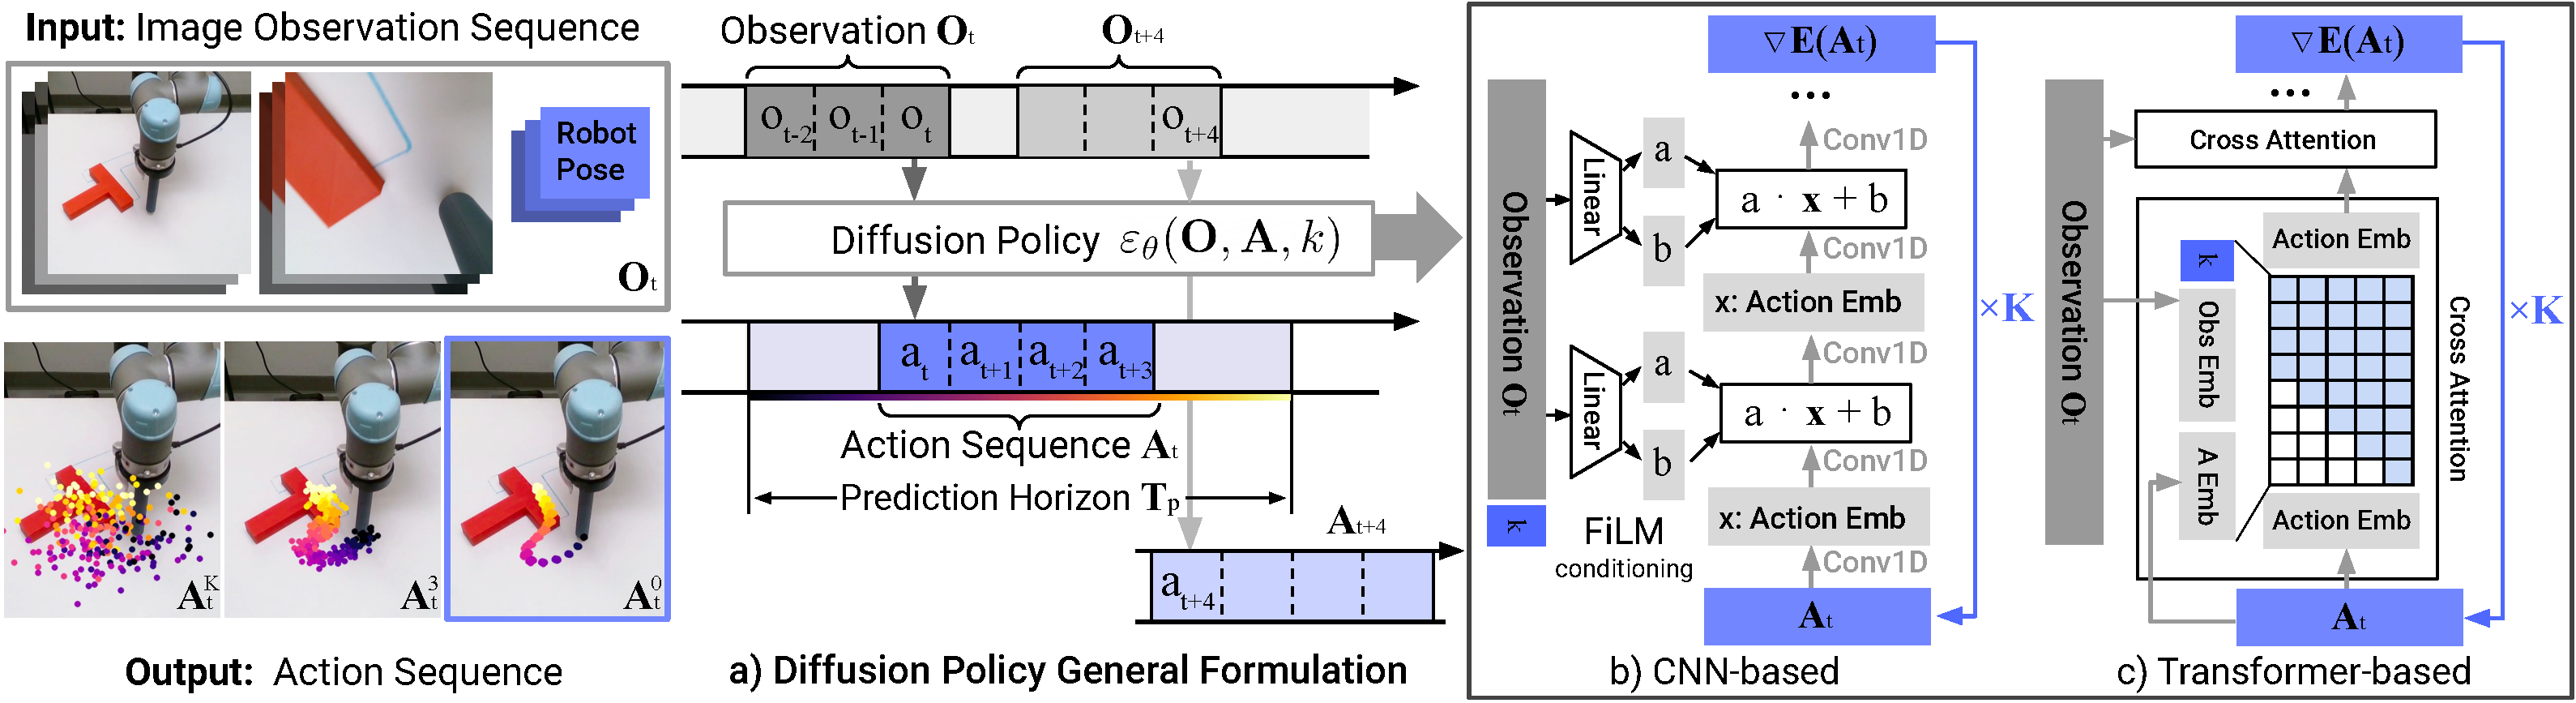
\includegraphics[width=\linewidth]{figures/policy_input_output.pdf}
    \caption{a) Denoising network overview, b) CNN-based and c) Transformer-based architectures.}
    \label{fig:diffusion_policy}
\end{figure*}
The first model is a 1D U-Net composed of strided and transposed convolutions, with conditioning
incorporated through FiLM layers. The second model includes attention layers and uses cross-attention
for conditioning.
The integration of the network within the diffusion process is shown in Figure \ref{fig:diffusion}.

\begin{figure}
    \centering
    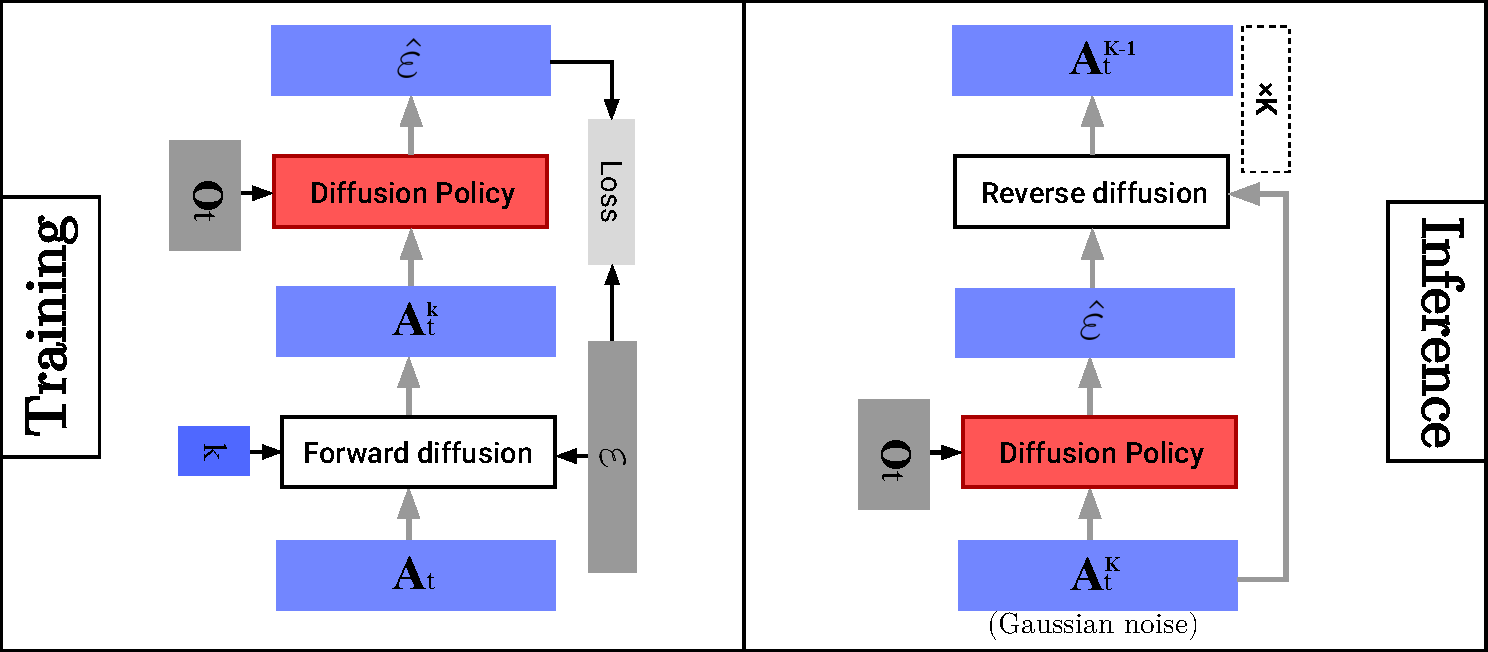
\includegraphics[width=\linewidth]{figures/diffusion.pdf}
    \caption{Diffusion involves training the network to denoise noisy action sequences,
    in order to be able to sample sequences from pure noise during inference.}
    \label{fig:diffusion}
\end{figure}
\begin{table}[!htb]
    \centering
    \begin{tabular}{c|c}
        \textbf{Method} & max / avg \\
        \hline
        LSTM-GMM & 0.69/0.54 \\
        IBC & 0.75/0.64 \\
        \textbf{DP-CNN} & \textbf{0.91}/\textbf{0.84} \\
        \textbf{DP-Transformer} & 0.78/0.66
    \end{tabular}
    \caption{Success rate in the PushT environment. The goal of the agent is to push a T-shaped
    block to a fixed target. The CNN version of DP outperforms its competitors.}
    \label{tab:success_rate}
\end{table}
The approach is evaluated on the PushT environment (Table \ref{tab:success_rate}).
DP has proven to be capable of modeling multimodal distributions (Figure \ref{fig:multimodality}).
\begin{figure}
    \centering
    \fbox{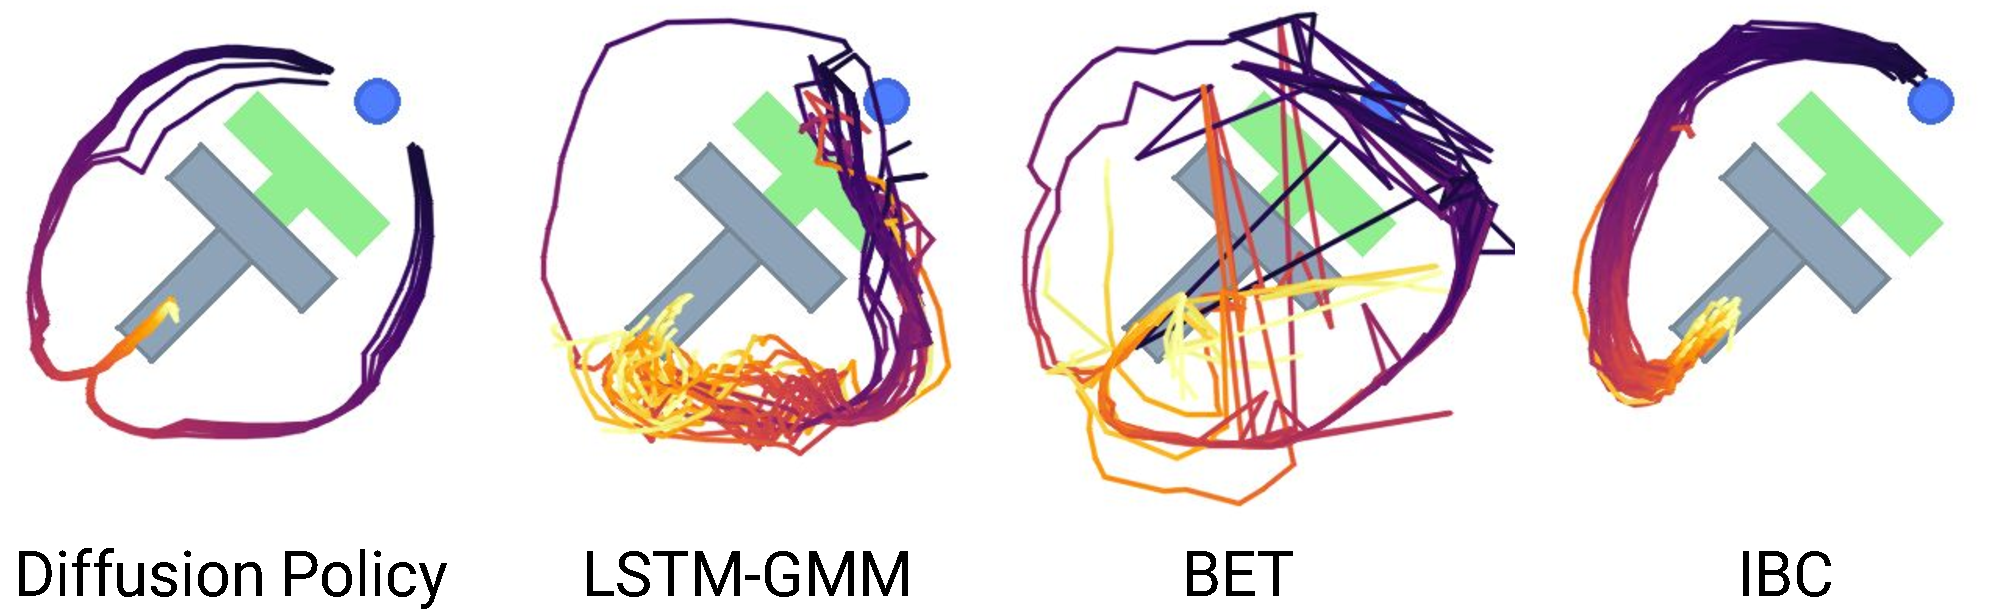
\includegraphics[width=\linewidth]{figures/multimodal_sim.pdf}}
    \caption{Ability of different approaches to handle multimodality. The agent (blue) must push the
    object (grey) to the target (green). In this specific case, the agent should be able to bypass the
    T-shaped obstacle by the left or right.}
    \label{fig:multimodality}
\end{figure}
